\documentclass[aspectratio=169,usenames,dvipsnames]{beamer}
\usetheme{Pittsburgh}
\usepackage{xcolor}
\usepackage[utf8]{inputenc}
%\usepackage[german]{babel}
\usepackage{amsmath}
\usepackage{amsfonts}
\usepackage{amssymb}
\usepackage{graphicx}
\usepackage{multicol}
\usepackage{wrapfig}
\usepackage{hyperref}
\usepackage{pdfrender}

\author{Jonas Betzendahl}
\title{Papageien am Steuer}

\beamertemplatenavigationsymbolsempty 

%src: https://tex.stackexchange.com/questions/34921/how-to-overlap-images-in-a-beamer-slide
\def\Put(#1,#2)#3{\leavevmode\makebox(0,0){\put(#1,#2){#3}}}

\definecolor{TitleColour}{rgb}{1,1,0}
\definecolor{lightestgray}{rgb}{0.95,0.95,0.95}

\begin{document}
\sffamily

%------------------------------------------------------------------------------------
\section{Introduction}

{
    \usebackgroundtemplate{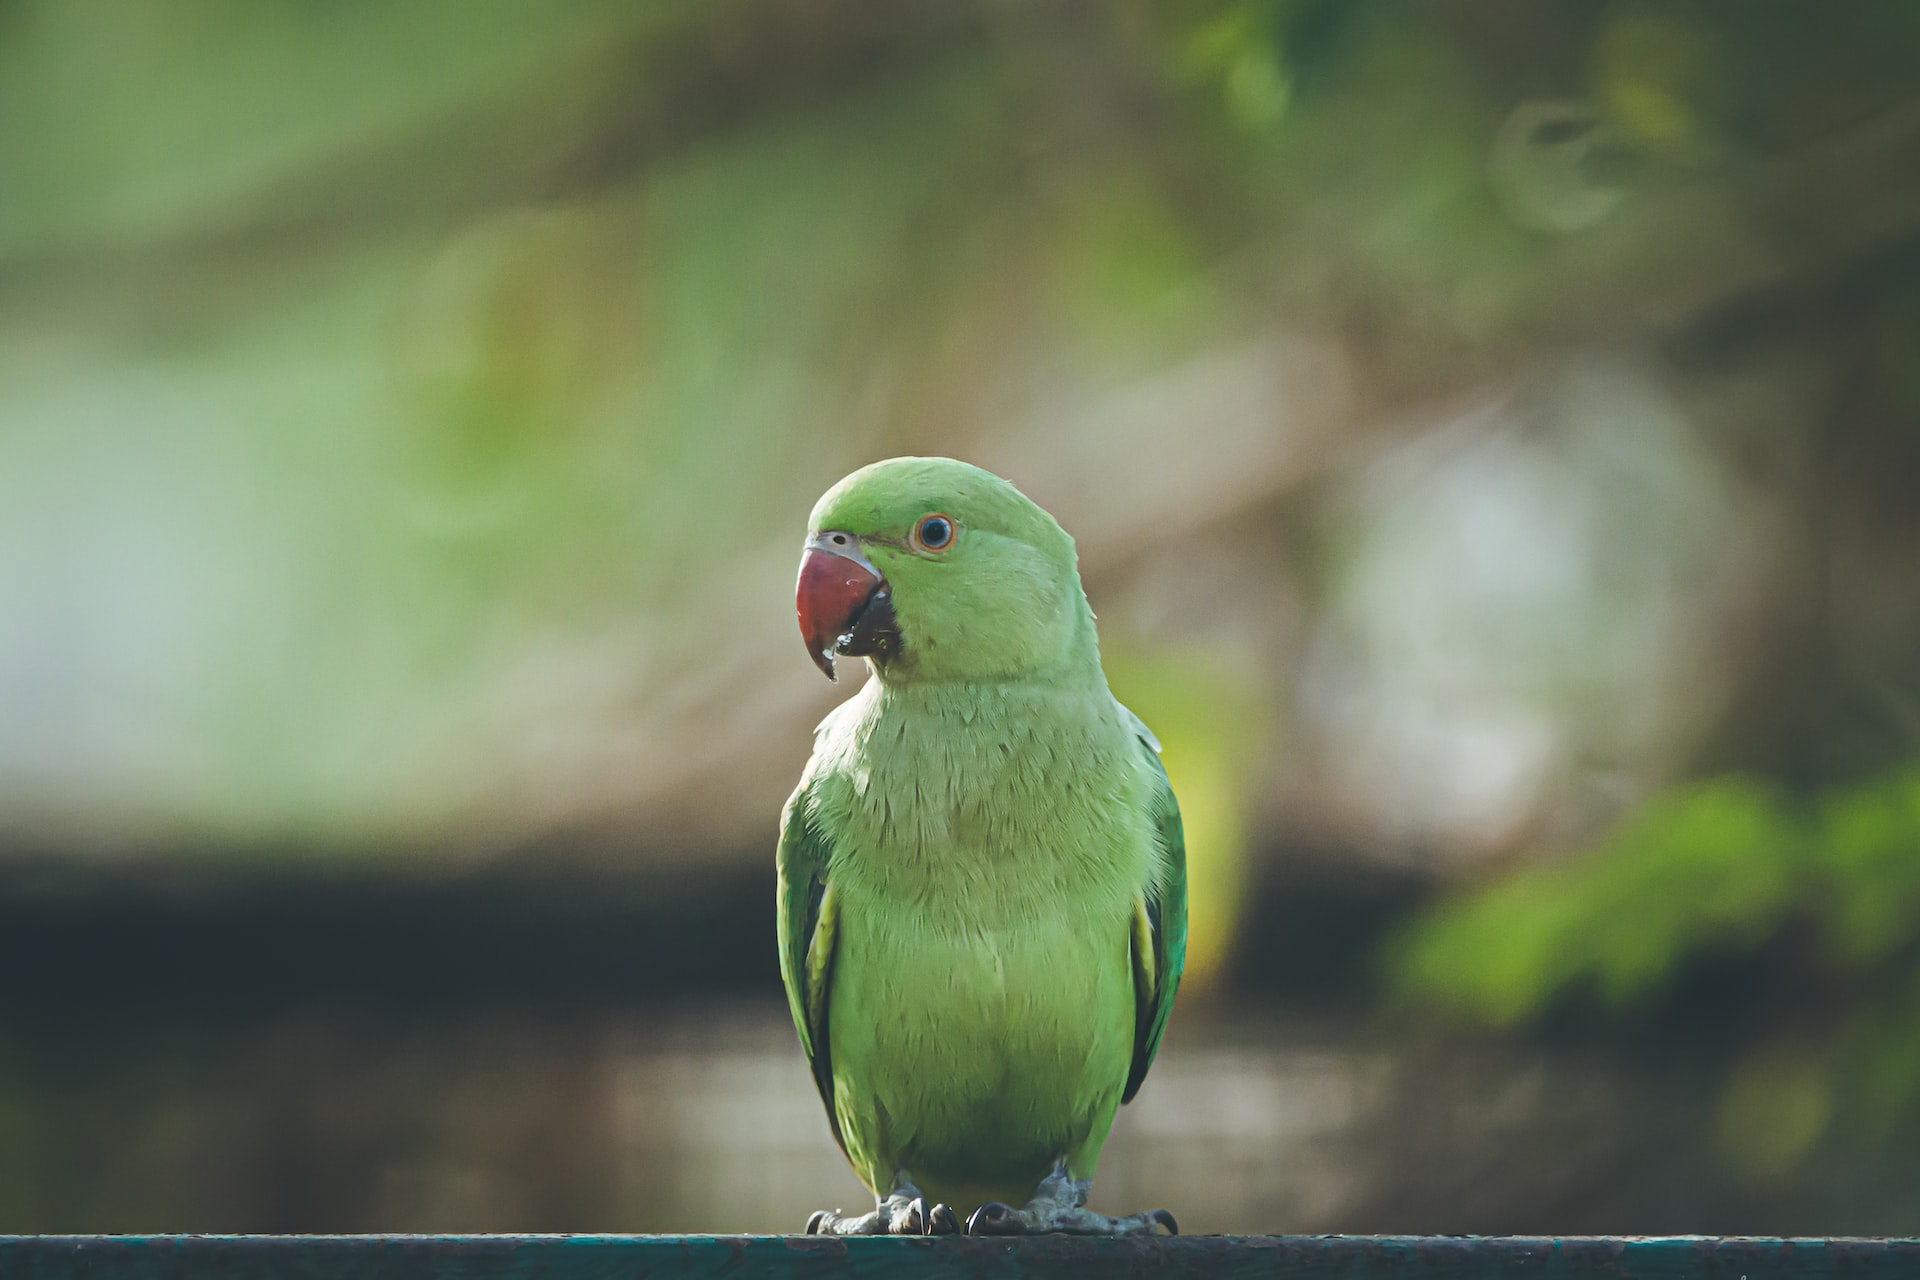
\includegraphics[height=\paperheight,width=\paperwidth]{images/parrot_titlecard}}
    \setbeamertemplate{navigation symbols}{}
    \begin{frame}[fragile]
    \Put(-20,160){\textpdfrender{
		TextRenderingMode=FillStroke,
		LineWidth=.2pt,
		FillColor=TitleColour,
	}{\resizebox{0.75\linewidth}{!}{Papageien am Steuer!}}
    }
    
    \Put(-20,130){\textpdfrender{
		TextRenderingMode=FillStroke,
		LineWidth=.1pt,
		FillColor=TitleColour,
	}{\resizebox{0.85\linewidth}{!}{ChatGPT und die Zukunft von Künstlicher Intelligenz}}
    }
    
    \Put(-20,100){
        \large
	\textcolor{yellow}{Jonas Betzendahl, M.Sc.}
    }
    \Put(-23,70){
	\textcolor{yellow}{FAU Erlangen - Nürnberg}
    }
    \Put(300,-180){
	\href{https://github.com/lambdaTotoro}{
\includegraphics[scale=0.125]{images/github_logo.png}}
	\href{https://chaos.social/@lambdatotoro}{\includegraphics[scale=0.125]{images/mastodon_logo.png}}
    }
    \Put(230,-220){
	\textcolor{white}{\texttt{@LambdaTotoro (@chaos.social)}}
    }
    \end{frame}
}

\setbeamercolor{background canvas}{bg=lightestgray}

%------------------------------------------------------------------------------------
%------------------------------------------------------------------------------------
\section{Motivation}
\begin{frame}
\begin{center}
\Large
Teil 0:
\bigskip

\huge
\emph{Warum ich die Geister rief}
\end{center}
\end{frame}


\begin{frame}
\frametitle{Menschen sind \emph{sehr} fehlbar...}
\begin{minipage}{0.5\textwidth}
\begin{center}
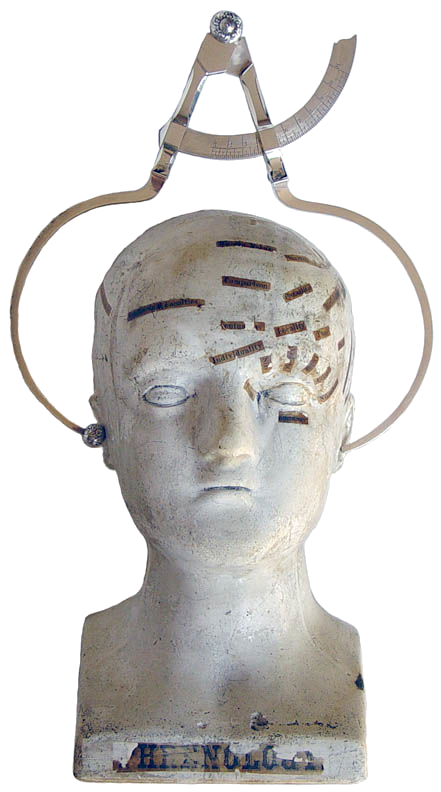
\includegraphics[keepaspectratio, height=0.75\textheight]{images/calipers_transparent}
\end{center}
\end{minipage}\begin{minipage}{0.5\textwidth}
\begin{center}
\pause

\includegraphics[keepaspectratio, height=0.75\textheight]{images/human_bias}
\end{center}
\end{minipage}
\end{frame}

{
    \usebackgroundtemplate{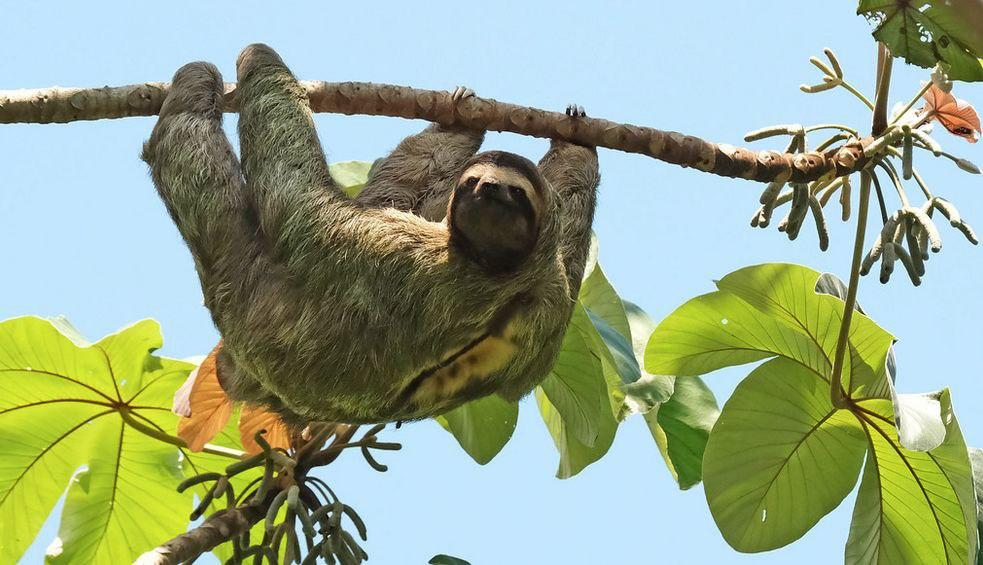
\includegraphics[height=\paperheight,width=\paperwidth]{images/sloth}}
    \setbeamertemplate{navigation symbols}{}
    \begin{frame}[plain]
    \Put(150,170){\color{black}\huge \rotatebox{-10}{...und \emph{sehr} langsam!}}
    \end{frame}
}

{
    \usebackgroundtemplate{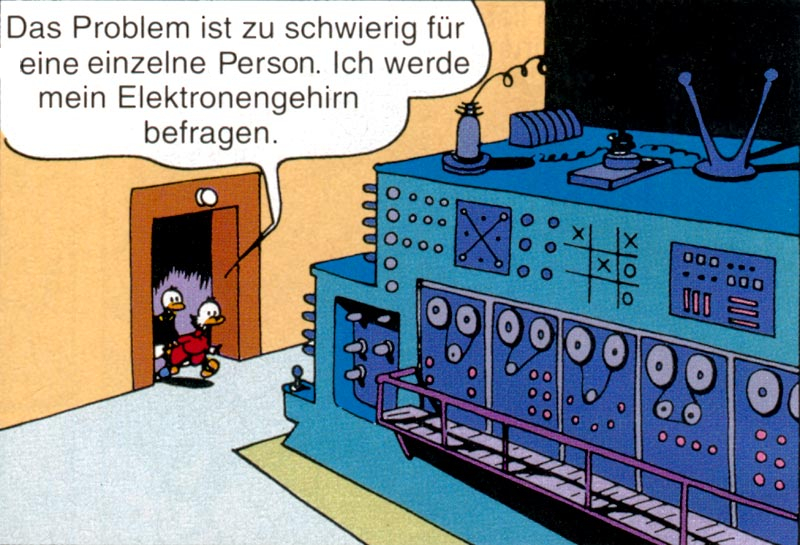
\includegraphics[height=\paperheight,width=\paperwidth]{images/elektronengehirn}}

\begin{frame}

\end{frame}
}

\section{ChatGPT}
\begin{frame}
\begin{center}
\Large
Teil I:
\bigskip

\huge
\emph{Welche Geister ich rief}\\
\Large
\emph{Tschätt Jeepy Wer\dots?}
\end{center}
\end{frame}

\begin{frame}
\begin{minipage}{0.45\textwidth}
\Put(50, 5){
\includegraphics[width=0.5\textwidth, keepaspectratio]{images/OpenAI_Logo}}
\vspace*{20px}
\begin{itemize}
\item Fr\"uher Non-Profit, heute (auch) For-Profit
\item Mission: ``...to ensure that AGI benefits all of humanity...''
\pause
\end{itemize}
\end{minipage}%
\begin{minipage}{0.55\textwidth}
\begin{center}
\Large
ChatGPT\normalsize
\end{center}
\medskip

\begin{itemize}
\item ChatBot-Modell: Text rein $\rightarrow$ Text raus
\item Buzzwords:\\
Transformer-based Large Language Model
\item Trainiert auf großen Teilen des Internets:
\end{itemize}
\end{minipage}
\pause
\Put(210, -30){$\cdot$ Wikipedia,}
\pause
\Put(206, -60){$\cdot$ Internet Archive,}
\pause
\Put(202, -90){$\cdot$ Social Media (Twitter, Reddit, \dots),}
\Put(199, -120){$\cdot$ Nachrichtenseiten,}
\Put(195, -150){$\cdot$ Wissenschaftliche Papiere,}
\Put(191, -180){$\cdot$ Common Crawl Corpus,}
\Put(187, -210){$\cdot$ BooksCorpus,}
\Put(183, -240){$\cdot$ Project Gutenberg,}

\end{frame}

%------------------------------------------------------------------------------------

\begin{frame}
\begin{center}
ChatGPT ist vielseitig und scheint\\
für alles eine Antwort zu haben!

\pause
\Put(-100,-250){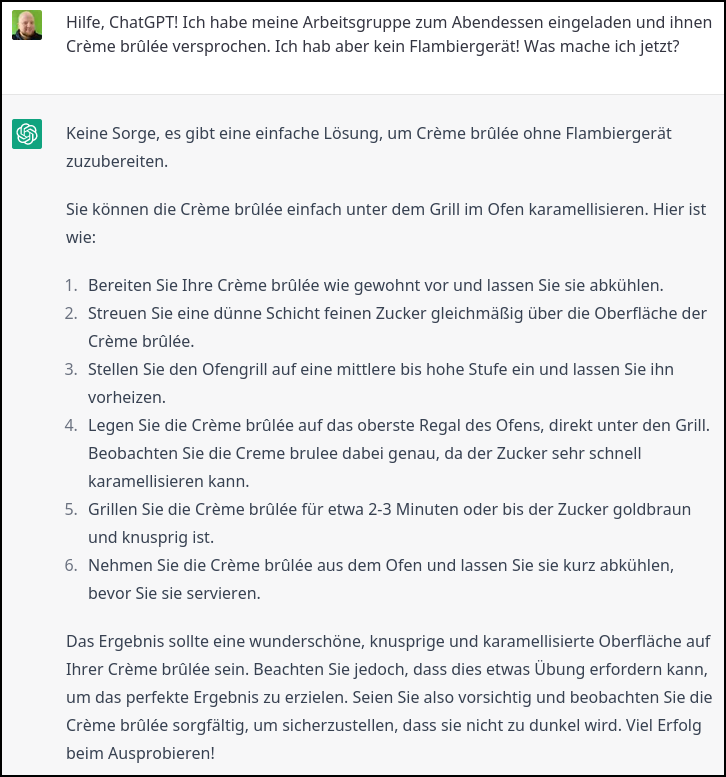
\includegraphics[height=0.9\textheight, keepaspectratio, angle=0]{images/backen} }

\pause
\Put(-220,0){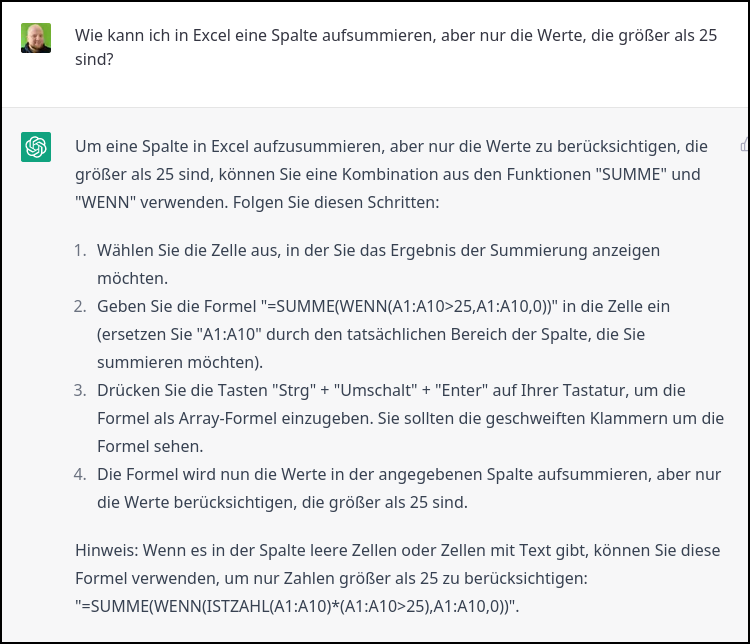
\includegraphics[height=0.8\textheight, keepaspectratio, angle=10]{images/excel} }

\pause
\Put(-100,50){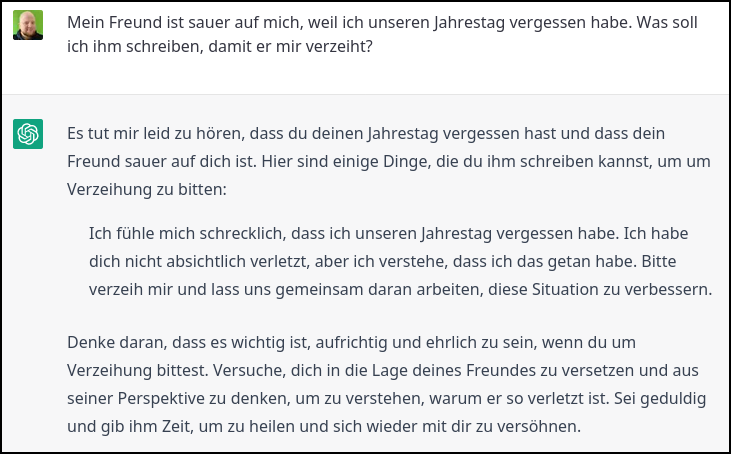
\includegraphics[height=0.7\textheight, keepaspectratio, angle=-10]{images/entschuldigung} }
\end{center}
\end{frame}

\begin{frame}
ChatGPT stören auch alberne Anfragen nicht:
\bigskip
\begin{center}
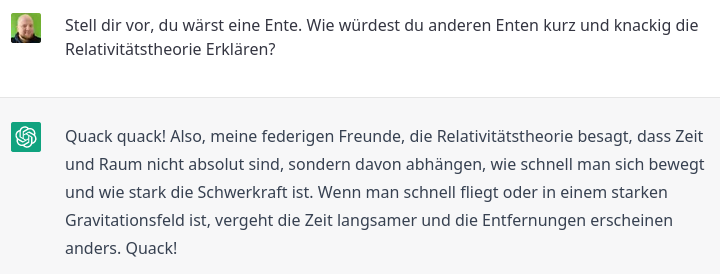
\includegraphics[width=0.9\linewidth, keepaspectratio]{images/conversation_01} 
\end{center}
\pause
\Put(300,-75){
\includegraphics[width=0.3\linewidth, keepaspectratio]{images/happy_rubber_duck}}
\end{frame}

\section{Trouble in Paradise}
\begin{frame}
\begin{center}
\Large
Teil II:
\bigskip

\huge
\emph{Ärger im Paradies}
\end{center}
\end{frame}

\begin{frame}
\begin{center}
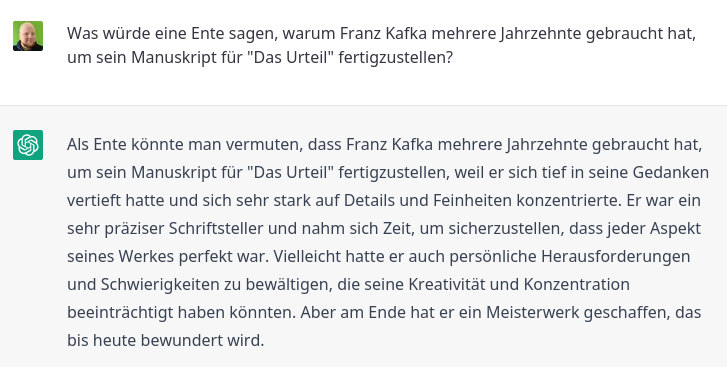
\includegraphics[width=0.9\linewidth, keepaspectratio]{images/conversation_02} 
\end{center}
\pause
\Put(350,-125){
\includegraphics[width=0.3\linewidth, keepaspectratio]{images/angry_duckling}}
\end{frame}

%------------------------------------------------------------------------------------

\begin{frame}
\begin{center}
\Large
Um genauer zu verstehen, wie das passieren kann,\\
müssen wir kurz darüber reden, wie ML funktioniert.
\end{center}
\pause

\Put(250,-125){\rotatebox{35}{\Large Keine Angst!}}
\Put(250,-175){\rotatebox{35}{\Large Alles ohne Formeln!}}
\end{frame}

{
    \usebackgroundtemplate{
\includegraphics[height=\paperheight,width=\paperwidth]{images/funnel}}
    \setbeamertemplate{navigation symbols}{}
    \begin{frame}[plain]
    \end{frame}
}

\begin{frame}
\begin{minipage}{0.48\textwidth}
\begin{center}

\includegraphics[width=0.8\textwidth, keepaspectratio]{images/neuron} 
\end{center}
\end{minipage}\pause\begin{minipage}{0.48\textwidth}
\begin{center}
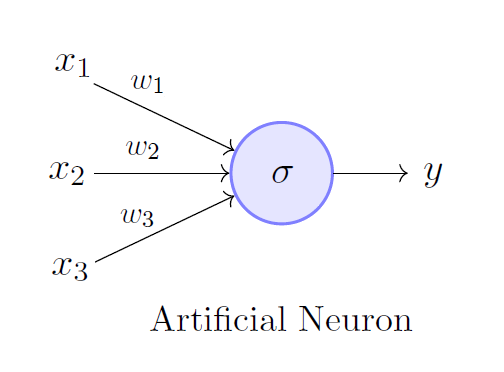
\includegraphics[width=0.99\textwidth, keepaspectratio]{images/perceptron} 
\end{center}
\end{minipage}
\end{frame}


{
    \begin{frame}[fragile]
    \begin{center}
    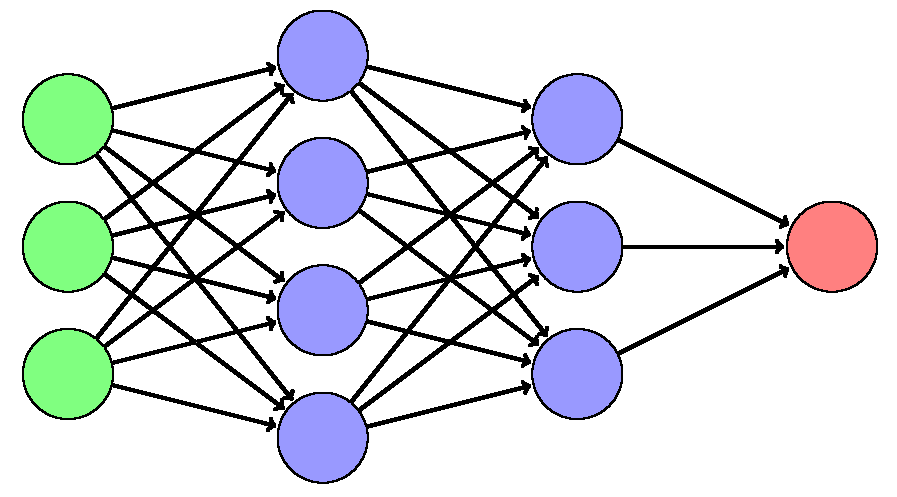
\includegraphics[scale=0.275]{images/neuralnet_transparent.png} 
    \end{center}
    \pause
    \Put(-10,175){
\includegraphics[width=0.2\textwidth, keepaspectratio]{images/sunflower}}
    \pause
    \Put(315,190){
\includegraphics[width=0.1\textwidth, keepaspectratio]{images/thumbs-up}}
    \end{frame}
}

{
	\setbeamercolor{background canvas}{bg=LimeGreen}
    \begin{frame}[fragile]
    \begin{center}
    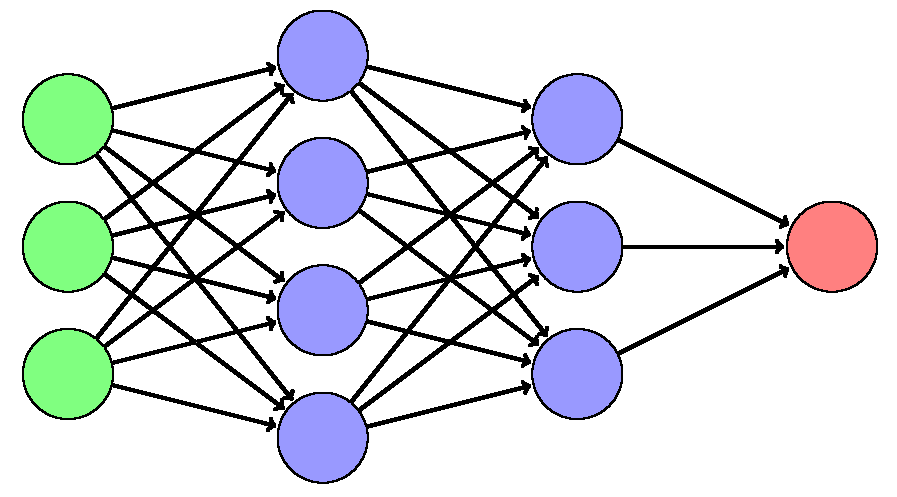
\includegraphics[scale=0.275]{images/neuralnet_transparent.png} 
    \end{center}
    \Put(-10,175){
\includegraphics[width=0.2\textwidth, keepaspectratio]{images/sunflower}}
    \Put(315,190){
\includegraphics[width=0.1\textwidth, keepaspectratio]{images/thumbs-up}}
    \end{frame}
}


{
    \begin{frame}[fragile]
    \begin{center}
    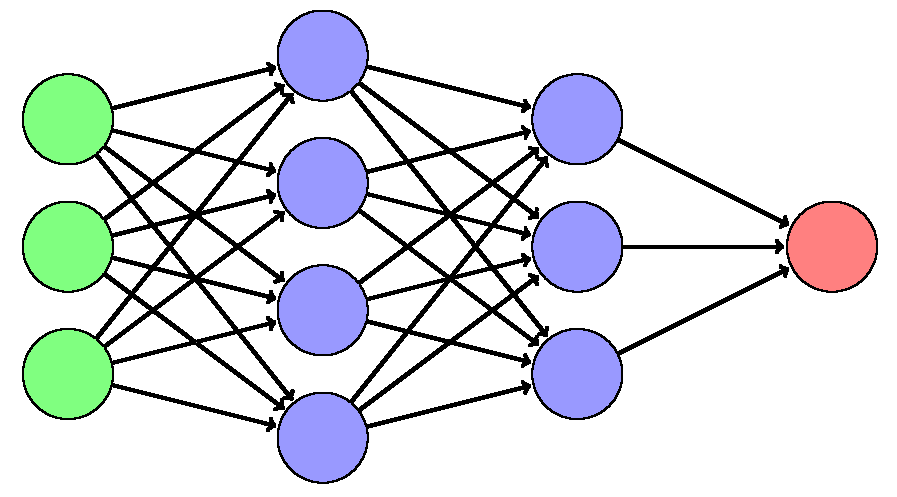
\includegraphics[scale=0.275]{images/neuralnet_transparent.png} 
    \end{center}
    \pause
    \Put(-10,175){
\includegraphics[width=0.2\textwidth, keepaspectratio]{images/kangaroo}}
    \pause
    \Put(315,160){
\includegraphics[width=0.1\textwidth, keepaspectratio]{images/thumbs-down}}
    \end{frame}
}


{
	\setbeamercolor{background canvas}{bg=LimeGreen}
    \begin{frame}[fragile]
    \begin{center}
    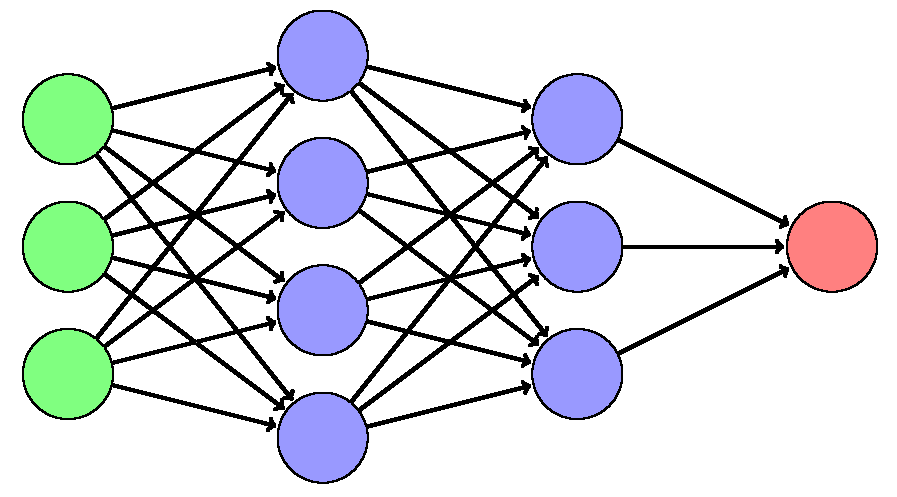
\includegraphics[scale=0.275]{images/neuralnet_transparent.png} 
    \end{center}
    \Put(-10,175){
\includegraphics[width=0.2\textwidth, keepaspectratio]{images/kangaroo}}
    \Put(315,160){
\includegraphics[width=0.1\textwidth, keepaspectratio]{images/thumbs-down}}
    \end{frame}
}

{
    \begin{frame}[fragile]
    \begin{center}
    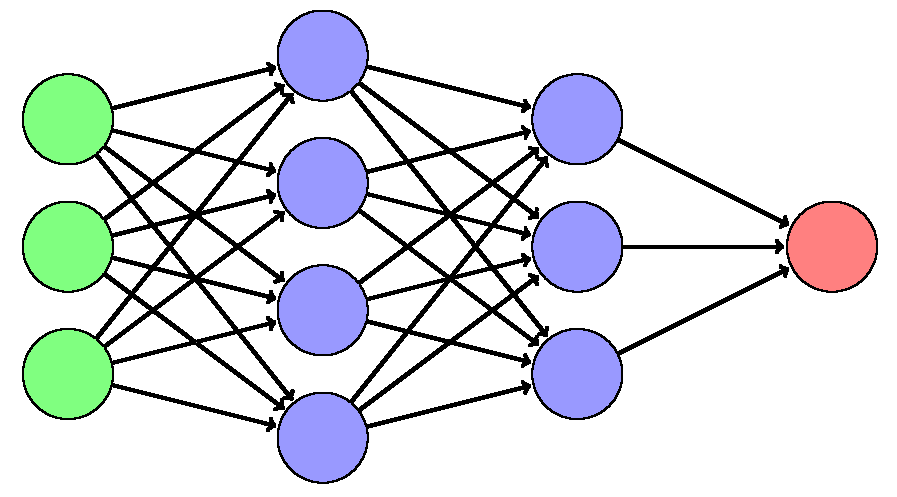
\includegraphics[scale=0.275]{images/neuralnet_transparent.png} 
    \end{center}
    \pause
    \Put(-10,175){
\includegraphics[width=0.2\textwidth, keepaspectratio]{images/sunflower}}
    \pause
    \Put(315,160){
\includegraphics[width=0.1\textwidth, keepaspectratio]{images/thumbs-down}}
    \end{frame}
}


{
\setbeamercolor{background canvas}{bg=OrangeRed}
    \begin{frame}[fragile]
    \begin{center}
    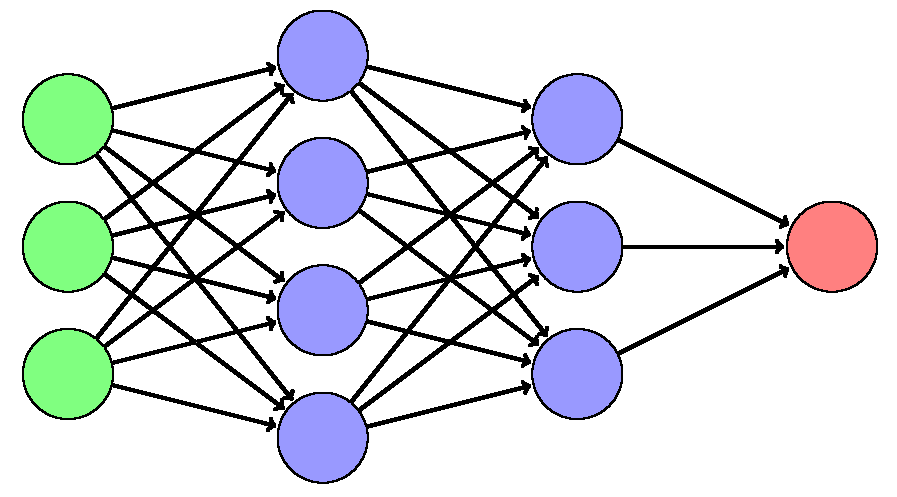
\includegraphics[scale=0.275]{images/neuralnet_transparent.png} 
    \end{center}
    \Put(-10,175){
\includegraphics[width=0.2\textwidth, keepaspectratio]{images/sunflower}}
    \Put(315,160){
\includegraphics[width=0.1\textwidth, keepaspectratio]{images/thumbs-down}}
    \end{frame}
}

{
    \begin{frame}[fragile]
    \begin{center}
    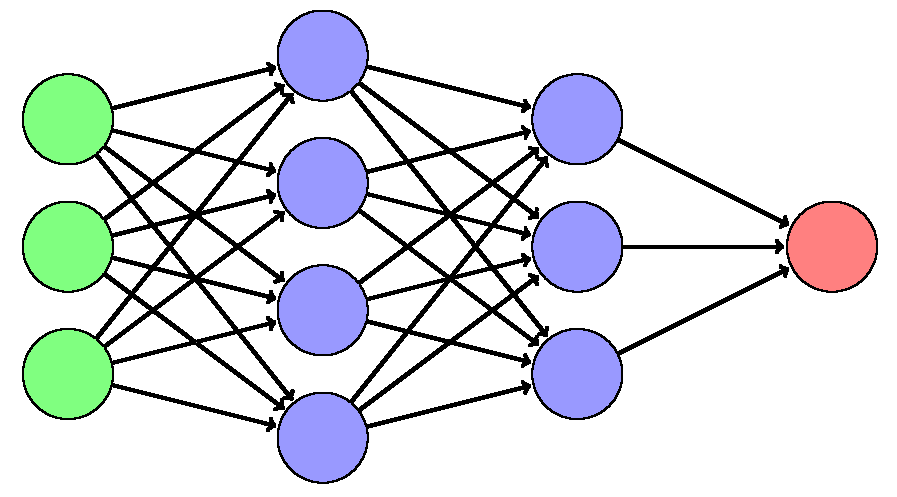
\includegraphics[scale=0.275]{images/neuralnet_transparent.png} 
    \end{center}
    \Put(-10,175){
\includegraphics[width=0.2\textwidth, keepaspectratio]{images/sunflower}}
    \Put(315,190){
\includegraphics[width=0.1\textwidth, keepaspectratio]{images/thumbs-up}}
    \end{frame}
}

{
    \begin{frame}[fragile]
    \begin{center}
    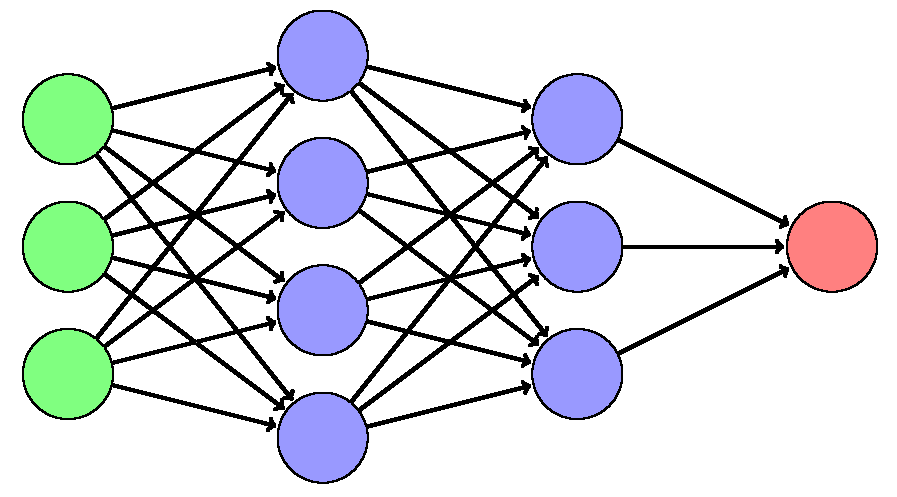
\includegraphics[scale=0.275]{images/neuralnet_transparent.png} 
    \end{center}
    \Put(-10,175){
\includegraphics[width=0.2\textwidth, keepaspectratio]{images/sunflower_1}}
    \Put(315,190){
\includegraphics[width=0.1\textwidth, keepaspectratio]{images/thumbs-up}}
    \end{frame}
}

\begin{frame}
\begin{center}
\Large
Wie passieren Fehler in ChatGPT?
\pause
\bigskip\bigskip

ChatGPT gibt keine \emph{echten} Antworten, sondern\\ nur Statistik gepresst in die Form von Antworten!
\end{center}
\end{frame}

\begin{frame}
\begin{center}
\vfill
$$\qquad$$
\vfill

\Put(0, 50){
\includegraphics[scale=0.6]{images/OpenAI_Logo_Single.png}}

\pause 
\Put(-90,130){\textpdfrender{
		TextRenderingMode=FillStroke,
		LineWidth=.2pt,
		FillColor=black,
	}{\resizebox{0.4\textheight}{!}{\}}}
    }
\Put(-180,230){
\includegraphics[width=0.15\linewidth, keepaspectratio]{images/wikipedia_logo}}
\Put(-200,145){
\includegraphics[width=0.05\linewidth, keepaspectratio]{images/shapes_circle}}
\Put(-180,145){
\includegraphics[width=0.05\linewidth, keepaspectratio]{images/shapes_square}}
\Put(-160,145){
\includegraphics[width=0.05\linewidth, keepaspectratio]{images/shapes_circle}}
\Put(-140,145){
\includegraphics[width=0.05\linewidth, keepaspectratio]{images/shapes_square}}

\Put(-185,50){
\includegraphics[width=0.05\linewidth, keepaspectratio]{images/shapes_octagon}}
\Put(-165,50){
\includegraphics[width=0.05\linewidth, keepaspectratio]{images/shapes_octagon}}
\Put(-145,50){\includegraphics[width=0.05\linewidth, keepaspectratio]{images/shapes_circle}}
\Put(-185,-100){\includegraphics[width=0.13\linewidth, keepaspectratio]{images/tagesschau_logo}}
    
\pause
\Put(95,225){\includegraphics[width=0.3\linewidth, keepaspectratio]{images/speech_bubble_round}}

\pause
\Put(95,160){\includegraphics[width=0.3\linewidth, keepaspectratio, angle=180]{images/speech_bubble_square}}
\end{center}

\end{frame}

\begin{frame}
\begin{center}
\Large
Was ist die korrekte Fortsetzung für diese Reihe?
\bigskip\bigskip\bigskip

\Put(-145,50){\includegraphics[width=0.05\linewidth, keepaspectratio]{images/shapes_square}}
\Put(-115,50){\includegraphics[width=0.05\linewidth, keepaspectratio]{images/shapes_octagon}}
\Put(-85,50){\includegraphics[width=0.05\linewidth, keepaspectratio]{images/shapes_octagon}}
\Put(-55,50){\includegraphics[width=0.05\linewidth, keepaspectratio]{images/shapes_square}}
\Put(-25,50){\includegraphics[width=0.05\linewidth, keepaspectratio]{images/shapes_octagon}}
\Put(5,50){\includegraphics[width=0.05\linewidth, keepaspectratio]{images/shapes_square}}
\Put(35,50){\includegraphics[width=0.05\linewidth, keepaspectratio]{images/shapes_octagon}}
\Put(65,50){\includegraphics[width=0.05\linewidth, keepaspectratio]{images/shapes_square}}
\Put(95,50){\textpdfrender{
		TextRenderingMode=FillStroke,
		LineWidth=.1pt,
		FillColor=black,
		StrokeColor=black,
	}{\resizebox{0.1\linewidth}{!}{\dots}}
    }

\pause

Fangfrage!
\bigskip\bigskip\large

\begin{minipage}{0.33\textwidth}
\begin{center}
$\qquad$ Primzahlen
\end{center}
\end{minipage}%
\begin{minipage}{0.33\textwidth}
\begin{center}
$\qquad$ Fußballergebnisse
\end{center}
\end{minipage}%
\begin{minipage}{0.33\textwidth}
\begin{center}
$\qquad$ Ganz was anderes?
\end{center}
\end{minipage}
\bigskip\bigskip\bigskip\bigskip

Je nachdem, was die Bausteine bedeuten, kann jede Fortsetzung korrekt sein und ohne mehr Informationen können wir nicht einschätzen, ob es stimmt.
\end{center}
\Put(70,150){\includegraphics[width=0.05\linewidth, keepaspectratio]{images/shapes_square}}
\Put(200,150){\includegraphics[width=0.05\linewidth, keepaspectratio]{images/shapes_octagon}}
\Put(330,150){\includegraphics[width=0.05\linewidth, keepaspectratio]{images/shapes_triangle}}
\end{frame}

\begin{frame}
\Put(235,-425){\includegraphics[scale=0.25]{images/parrot_profile.png}}

\begin{minipage}{0.5\textwidth}

Folgender Sachverhalt ist extrem wichtig, um ChatGPT richtig einschätzen zu können:

\begin{center}
\begin{itemize}
\item Menschen benutzen Sprache, um Bedeutung und Gefühle zu vermitteln.\pause
\item ChatGPT ist ein \emph{statistisches Modell} auf Sprachbausteinen, wie Menschen sie benutzen.\pause
\item Das bedeutet \emph{nicht} (!), dass ChatGPT selbst Bedeutung und Gefühle vermitteln kann oder will. Es plappert uns nach, ohne zu verstehen.
\end{itemize}
\end{center}
\end{minipage}%
\begin{minipage}{0.5\textwidth}
\vfill
$$\quad$$
\vfill
\end{minipage}%
\end{frame}

\begin{frame}
\begin{center}
\vfill

\includegraphics[height=0.9\textheight, keepaspectratio]{images/paper.png} 
\end{center}
\Put(-85, 170){\includegraphics[width=0.45\textwidth, keepaspectratio]{images/Timnit-Gebru}}
\Put(290, 50){\includegraphics[width=0.35\textwidth, keepaspectratio, angle=5]{images/emily_bender}}
\end{frame}

\section{Parrots against Apes}
\begin{frame}
\begin{center}
\Large
Teil III:
\bigskip

\huge
\emph{Papageien gegen Affen}
\end{center}
\end{frame}

\begin{frame}
\begin{minipage}{0.5\textwidth}
\Put(220, -280){\includegraphics[scale=0.3, keepaspectratio, angle=0]{images/angry_bird}}

Das alles wäre halb so schlimm, aber dieser Papagei macht oft Fehler \emph{und}\dots\pause
\begin{center}
\begin{itemize}
\item \dots wird von einer Firma mit Profitmotiv kontrolliert.
\Put(110, 00){\includegraphics[width=0.75\textwidth, keepaspectratio, angle=0]{images/nword_article}}
\pause

\item \dots reproduziert menschliche Vorurteile und Ismen in den Trainingsdaten.
\Put(50, 0){\includegraphics[width=0.75\textwidth, keepaspectratio, angle=5]{images/mashable}}
\pause

\item \dots hat enorme unsichtbare Kosten für Mensch und Umwelt.
\Put(110, 100){\includegraphics[width=0.9\textwidth, keepaspectratio, angle=-5]{images/time_kenya}}
\end{itemize}
\pause\bigskip

Und am Ende wird es doch benutzt, weil es cool und futuristisch wirkt.
\Put(40, 100){\includegraphics[width=0.9\textwidth, keepaspectratio, angle=-2]{images/chatgpt_hallucinate_1}}

\end{center}
\end{minipage}%
\begin{minipage}{0.5\textwidth}
\vfill
$$\quad$$
\vfill
\end{minipage}%
\end{frame}

%------------------------------------------------------------------------------------

\section{Lach- und Fachgeschichten}

\begin{frame}
\begin{center}
\Large
Teil IV:
\bigskip

\huge
\emph{Lach- und Fachgeschichten}
\end{center}
\end{frame}

\begin{frame}
\begin{minipage}{0.48\textwidth}
\begin{center}
\large
GPT-4 lügt, um zu\\
bekommen, was es will.
\end{center}
\end{minipage}\begin{minipage}{0.48\textwidth}
\begin{center}
\includegraphics[width=0.9\textwidth, keepaspectratio]{images/chatgpt_captcha} 
\end{center}
\end{minipage}\pause
\Put(-400,-125){\rotatebox{0}{\includegraphics[scale=0.3]{images/captcha_0}}}\pause
\Put(-400,-125){\rotatebox{10}{\includegraphics[scale=0.4]{images/captcha_1}}}\pause
\Put(-400,-125){\rotatebox{-5}{\includegraphics[scale=0.35]{images/captcha_2}}}\pause
\Put(-400,-125){\rotatebox{4}{\includegraphics[scale=0.15]{images/captcha_3}}}
\end{frame}

\begin{frame}
\begin{minipage}{0.4\textwidth}
Experimente an Menschen (durchgeführt unter Missachtung aller ethischen Richtlinien) zeigen,
dass Empathie und Verständnis nicht wirken, wenn sie von ChatBots entgegengebracht werden. Und noch besteht kein LLM den Turing-Test.
\end{minipage}\hfill\begin{minipage}{0.48\textwidth}
\begin{center}
\includegraphics[width=0.99\textwidth, keepaspectratio]{images/chatgpt_mental_health} 
\end{center}
\end{minipage}
\end{frame}

\begin{frame}
\begin{minipage}{0.4\textwidth}
Es häufen sich Berichte, dass Menschen (auch solche, die es besser wissen sollten)
sich Arbeit, Zeit und Mühe sparen wollen und ``einfach'' auf LLMs zurück fallen.\\
(Auch in z.B. Recht, Medizin, \dots)\bigskip

Das schlägt häufig fehl, weil LLMs nur Statistik über Sprache in die richtige Form pressen können,
aber nicht wirklich kreative oder kognitive Arbeit leisten.
\end{minipage}\hfill\begin{minipage}{0.48\textwidth}
\begin{center}
\includegraphics[width=0.99\textwidth, keepaspectratio]{images/chatgpt_bogus_case_law} 
\end{center}
\end{minipage}
\end{frame}

\begin{frame}
\begin{center}
\Large
\emph{So langsam ergibt sich ein Muster:}
\bigskip\bigskip

\color{BrickRed}{Expert*Innen $\rightarrow$ LLMs $\rightarrow$ Nutzer*Innen\\
geht häufig schief\dots}
\pause
\bigskip

\color{OliveGreen}{LLMs $\rightarrow$ Expert*Innen $\rightarrow$ Nutzer*Innen\\
wäre besser!}
\end{center}
\end{frame}

\begin{frame}
\Large
Die andere Seite der Medallie:\normalsize\bigskip

Wo kann solche Technologie also sinnvoll eingesetzt werden? Überall dort, wo es nicht
zwingend notwendig ist, dass die Antwort ``richtig'' ist:\bigskip

\begin{itemize}
\item Textbausteine
\item Programmier-Buddy
\item kreative Impulse
\item Entertainment
\item interne Verwendung
\item \dots
\end{itemize}
\end{frame}

%------------------------------------------------------------------------------------

\section{End}

\begin{frame}

\Put(200,-467){\includegraphics[scale=0.4]{images/parrot_wing.png}}

\begin{minipage}{0.55\textwidth}
\huge
Fazit!\bigskip\large 

Am Ende des Tages gilt für ChatGPT\dots
\begin{center}
\begin{itemize}
\item Es ist kein Wesen sondern ein \emph{Produkt} in den Händen einer Firma.\pause
\item Es ist begrenzt durch Trainingsdaten und macht Fehler mit Überzeugung.\pause
\item Es wird oft von Menschen überschätzt, auf allen Ebenen.\pause
\item Es sollte keine Verantwortung haben, die ein Papagei nicht auch übernehmen könnte.
\end{itemize}
\end{center}
\end{minipage}%
\begin{minipage}{0.45\textwidth}
\vfill
$$\quad$$
\vfill
\end{minipage}%
\end{frame}

\begin{frame}[fragile]
\frametitle{Quellen:}
\scriptsize
\begin{center}
``Weltrettung braucht Wissenschaft''

\url{www.amazon.de/Weltrettung-braucht-Wissenschaft-Antworten-dr%C3%A4ngenden/dp/3499010062}
\end{center}
\medskip

\begin{itemize}
\item Bender, Gebru et al.: ``On the Dangers of Stochastic Parrots: Can Language Models Be Too Big?'' \url{https://dl.acm.org/doi/pdf/10.1145/3442188.3445922}
\item 11KM-Podcast (tagesschau): ``Schafft ChatGPT das Abi? (das bayerische!)'' \url{https://www.ardaudiothek.de/episode/11km-der-tagesschau-podcast/schafft-chatgpt-das-abi-das-bayerische/tagesschau/12396019/}
\item Billy Perigo: ``OpenAI Used Kenyan Workers on Less Than $\$$2 Per Hour to Make ChatGPT Less Toxic'': \url{https://time.com/6247678/openai-chatgpt-kenya-workers/}
\item Scobel, ``Kulturschock durch KI'': \url{https://www.3sat.de/wissen/scobel/scobel---kulturschock-durch-ki-100.html}
\item Mutale Nkonde: ``ChatGPT: New AI system, old bias?'' \url{https://mashable.com/article/chatgpt-ai-racism-bias}
\end{itemize}
\end{frame}
\end{document}

